 \section{Propuesta de solución}
Se propone el desarrollo de un sistema integrado, completo y fácil de usar que procese, analice y visualice de forma eficiente datos de diversas fuentes, centrándose en los patrones de quietud sísmica \cite{SSN}~\cite{mcnally1983seismic}~\cite{wyss1997cannot}~\cite{scholz1997whatever}, las anomalías del campo eléctrico~\cite{varotsos1984physical}~\cite{yepez1995electric}, las anomalías del campo magnético~\cite{hayakawa1999fractal}~\cite{hayakawa2007monitoring} y las señales ionosféricas~\cite{eftaxias2003experience} como precursores específicos. Esta solución implicará varias etapas, incluyendo la recolección de datos muestreados y/o reportados, útiles para la implementación de algoritmos y así establecer patrones de comportamiento. 

 De acuerdo a lo ya mencionado anteriormente se propone:  

 \begin{figure}[H]
    \centering
    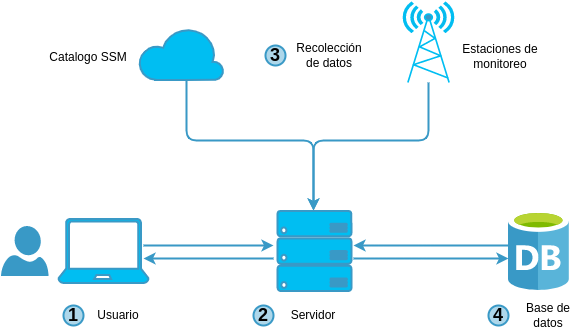
\includegraphics[width=0.8\textwidth]{img/arquitectura.drawio.png}
    \caption{Propuesta de interacción de actores del sistema}
    \label{fig:Arquitectura del sistema}
\end{figure}

\begin{itemize}
\item Visualización de los datos: \\
Los datos procesados deben presentarse en un formato gráfico para facilitar su interpretación. La integración de todos los componentes, desde la adquisición de datos hasta la visualización en un sistema podría implicar la creación de una aplicación web, software de escritorio u otras interfaces de usuario para mostrar las visualizaciones y permitir a los usuarios interactuar con el sistema. Adicionalmente hay que identificar los requisitos de visualización lo cual implica determinar los tipos de visualización necesarios, como gráficos, tablas o mapas. Elegir una biblioteca o herramienta de visualización tales como Ploty, Dygraphs y bokeh para visualizaciones basadas en web.
\\
\item Servidor:\\
Los datos recogidos se someterán a métodos y técnicas de caracterización para identificar patrones y correlaciones entre los distintos tipos de datos precursores.  Los datos almacenados se procesarán y analizarán para extraer información significativa. Este proceso implicará el uso de métodos estadísticos avanzados de análisis de patrones de sismicidad, análisis de correlaciones temporales y  fractalidad de los datos muestreados para usar algoritmos de procesamiento conocidos de comportamiento que se centren en los precursores específicos mencionados anteriormente. 
\\
\item Recolección de datos: \\
Para obtener los catálogos del Servicio Sismológico Nacional (datos para quietud sísmica), se utilizarán técnicas de web scraping. Este proceso implica el uso de herramientas y técnicas de programación para extraer datos de manera automatizada desde una página web \cite{SSN} o bien un servicio de almacenamiento en la nube (como Google Drive o Dropbox) para las estaciones de monitoreo. Los datos adquiridos se almacenarán en una base de datos como se muestra en el inciso 4 de la figura \ref{fig:Arquitectura del sistema}. Además, se pueden incluir datos complementarios, como el clima, la fase lunar y los macrosismos de otras partes del mundo para revisar la correlación con los ocurridos en México. Para identificar las tareas de procesamiento y análisis, es necesario determinar las tareas específicas necesarias, como la limpieza, el filtrado, la agregación y el análisis estadístico. Para esto, se pueden utilizar bibliotecas o marcos de trabajo como Pandas, NumPy o SciPy para el procesamiento de datos basado en Python. Por último, es necesario implementar el procesamiento y el análisis, lo que implica escribir código para realizar las tareas necesarias en los datos almacenados.
\item Almacenamiento de datos:\\
Una vez adquiridos los datos, hay que almacenarlos en una base de datos para su posterior procesamiento y análisis. Elegir una base de datos adecuada en función del formato de los datos y de los requisitos. Puede ser una base de datos relacional (por ejemplo, PostgreSQL, MySQL) o una base de datos NoSQL (por ejemplo, MongoDB, Cassandra) en función de la estructura de los datos y las necesidades de escalabilidad.Finalmente definir la estructura de las tablas o colecciones de la base de datos, especificando los campos y sus tipos de datos. 

\end{itemize}